\ChapterImagePrelim[cap:cronograma]{Cronograma}{./images/fondo.png}\label{cap:cronograma}
\mbox{}\\
\noindent

El cronograma (véase figura \ref{fig:cronograma}) organiza el desarrollo del proyecto Notación para el Diseño de Infraestructura de \TI (\NDITI): una propuesta desde la Universidad del Quindío durante el segundo semestre de 2025. 

El plan de trabajo se organiza en siete fases secuenciales y una actividad transversal, distribuidas a lo largo de 24 semanas (seis meses). La primera fase, orientada al reconocimiento de necesidades sobre el modelado de infraestructura de \TI, se desarrolla durante el primer mes y sirve como base para la formulación de la propuesta. 

En los meses siguientes se avanza con la identificación y caracterización de notaciones candidatas a~\NDITI~(meses 2 y 3), proceso que permite establecer criterios de selección y evaluación. Posteriormente, durante el cuarto mes, se ejecuta el análisis \DAR, mediante el cual se determina la notación de referencia que sustenta la propuesta final.

El quinto mes está dedicado al diseño y especificación de la notación NDITI, integrando los resultados conceptuales y técnicos obtenidos en las fases previas. Finalmente, el sexto mes se destina a la validación de la propuesta mediante ejemplos de modelado y análisis de aplicabilidad en contextos académicos. La construcción del documento final se desarrolla de forma transversal a lo largo de todo el periodo de ejecución, registrando avances, decisiones y resultados del proyecto.

\begin{figure}[H]
	\centering
	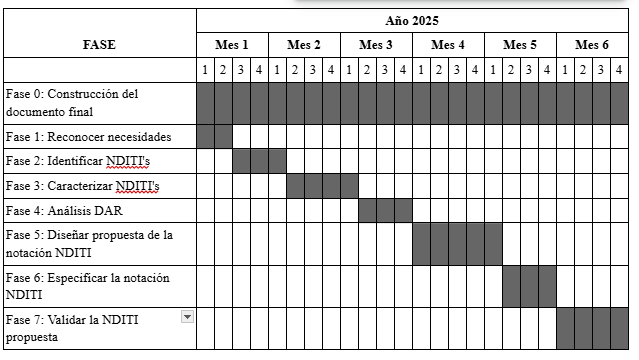
\includegraphics[scale=0.5]{tablas-images/partes/01-generalidades/cronograma.png}
	\caption{Cronograma de actividades del proyecto.}\label{fig:cronograma}
\end{figure}
